\documentclass[../Dokumentacja.tex]{subfiles}
\begin{document}
\subsection{Agent PU}
Agent jest graczem w \textbf{The Project Game}. Należy do jednej z dwóch drużyn. Integruje się z modułem \textbf{Game Master} poprzez moduł \textbf{Serwera Komunikacyjnego}. Przed wykonaniem jakichkolwiek akcji musi dołączyć do rozgrywki wysyłając odpowiednie zapytanie do GM. Posiada ograniczoną wiedzę na temat aktualnego stanu planszy i może ją zdobywać poprzez wykonywanie akcji oraz przez wymianę informacji z innymi graczami, zatem jego wiedza może być nieprawdziwa. Z tego powodu, aby wykonać jakąkolwiek akcję, agent musi uprzednio odpytać o nią GM, który posiada pełną wiedzę na temat aktualnego stanu planszy i może sprawdzić poprawność i wynik akcji. Celem Agenta jest wygrana drużyny do której należy, poprzez realizację obranej strategii.

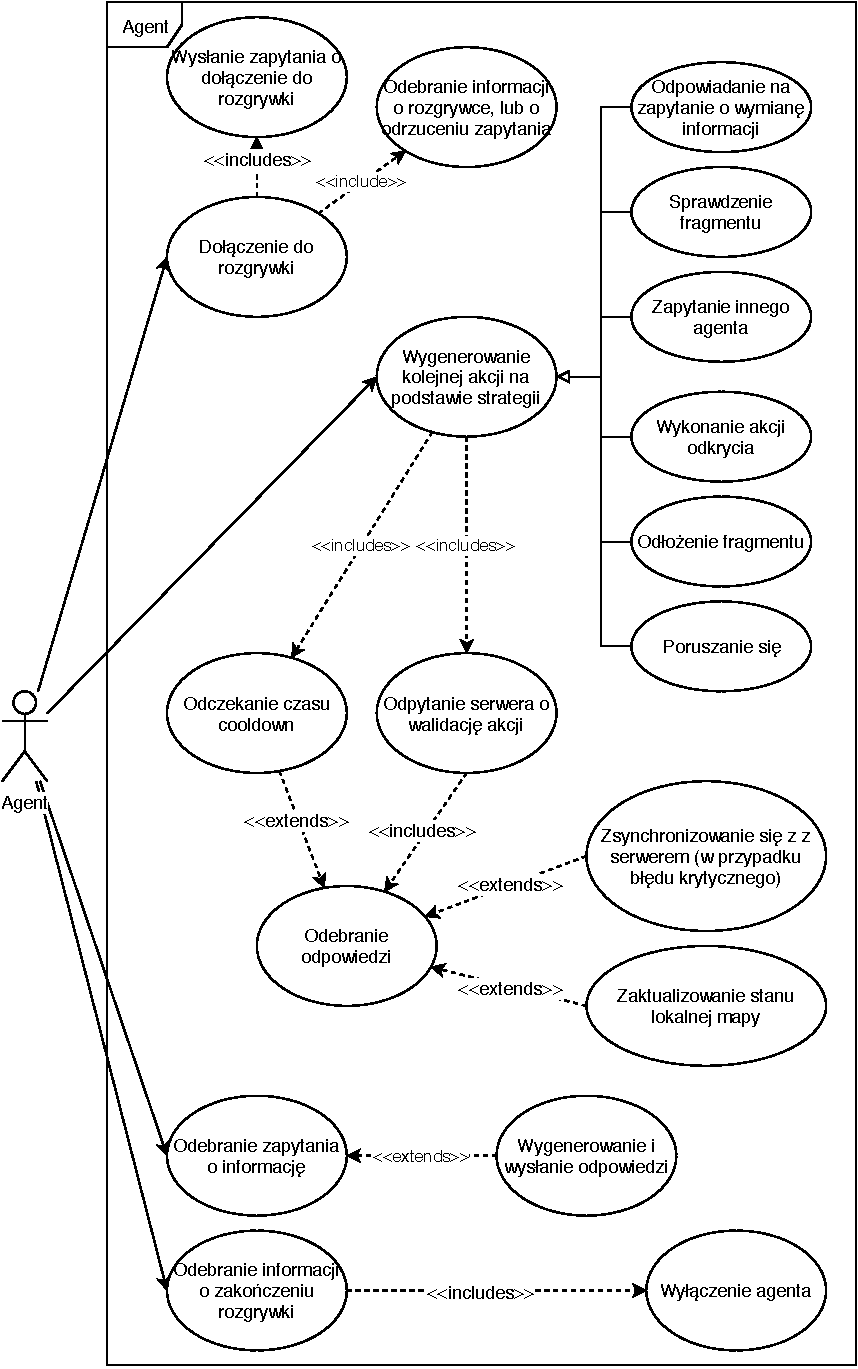
\includegraphics[width=\textwidth]{resources/Agent-Agent.pdf}

\begin{itemize}
    \item Dołączenie do rozgrywki
    \begin{itemize}
        \item Odbywa się poprzez połczenie się z Serwerem Komunikacyjnym na podstwaie danych połączenia wprowadzonych przez użytkownika i wykonanie odpowiedniego zapytania do GM, jeśli połączenie nie powiodło się, Agent kończy działanie
        \item Odpowiedź zwrotna może być negatywna, w tym przypadku Agent kończy działanie
        \item W przypadku odpowiedzi pozytywnej, Agent aktualizuje swoje informacje o parametrach rozgrywki na podstawie informacji otrzymanych z GM i przystępuje do oczekiwania na informację o rozpoczęciu rozgrywki, podczas którego nie wykonuje żadnych czynności.
    \end{itemize}

    \item Trwająca rozgrywka
    \begin{itemize}
        \item Agent może wygenerować akcję no podstawie swojej strategii, przed wysłaniem zapytania do GM, powinien uprzednio odczekać czas kary nałożony przez GM w ramach wykonanie poprzedniej akcji, w przeciwnym przypadku otrzyma odpowiedź o błędzie od GM
        \item W zależności od typu akcji agent generuje różne rodzaje zapytań do GM. Akcje niewymagające przesyłania dodatkowych informacji do GM to: odłożenie fragmentu, sprawdzenie fragmentu, oraz wykonanie akcji odkrycia. Zapytanie o ruch wymaga wyspecyfikowania kierunku, zapytanie o wymianę informacji wymaga wyspecyfikowania id pytanego gracza, a odpowiedź na wymianę informacji wymaga wyspecyfikowania wiedzy agenta.
        \item Na każde zapytanie agent otrzymuje odpowiedź, którą powinien odebrać i zinterpretować, na podstawie nich Agent może zaktualizować stan swojej wiedzy o planszy. Jeśli była to odpowiedź o błędzie, Agent może na podstawie jej zawartości zsynchronizować się z GM.
        \item W trakcie trwającej rozgrywki Agent może otrzymać zapytanie o udzielenie informacji. W takim przypadku powinien, albo odpowiedzieć na takie zapytanie natychmiastowo, lub odłożyć taką odpowiedź na później i wysłać ją w ramach wygenerowania akcji na podstawie strategii. Jeśli zapytanie zostało wysłane przez lidera, odpowiedź jest obligatoryjna i agent powinien odpowiedzieć na takie zapytanie natychmiastowo.
    \end{itemize}
    \item Zakończenie rozgrywki
    \begin{itemize}
        \item W trakcie rozgrywki Agent może otrzymać informację o jej zakończeniu. W przypadku takiej informacji, niezależnie od powodu zakończenia rozgrywki, Agent powinien zakończyć działanie.
        \item Informacją o zakończeniu rozgrywki jest zarówno specjalna wiadomość wygenerowana przez GM, jak i każda informacja o błędzie połączenia, nie są prowadzone ponowne próby połączenia.
    \end{itemize}
\end{itemize}
\end{document}
